\documentclass[10pt,a4paper]{article}
\usepackage[T1]{fontenc}
\usepackage[utf8]{inputenc}
\usepackage[spanish,es-tabla]{babel}
\parindent=0cm %Modificar tamaño de sangria
\usepackage{amsmath}
\usepackage{amssymb,amsfonts,latexsym,cancel}
\usepackage{graphicx}
\usepackage{epstopdf}
\usepackage{float}
\usepackage{subfigure}
\usepackage{array}
\usepackage{longtable}
\newcolumntype{E}{>{$}c<{$}}
\setcounter{MaxMatrixCols}{40}
\usepackage{bm}
\usepackage{xcolor}
%%%%%%%%%%%%%%%%%%%%%%%%%%%%%%%%%%%%%
%%%PAQUETES O CONFIGURACION NUEVA%%%%
%%%%%%%%%%%%%%%%%%%%%%%%%%%%%%%%%%%%%
\usepackage[lmargin=2cm, rmargin=2cm,top=2.5cm,bottom=2cm]{geometry}
\usepackage{fancyhdr}
\pagestyle{fancy}
\fancyhead{}%%Es para limpiar el documento
\fancyhead[C]{GO}
\fancyhead[R]{
\includegraphics[scale=0.07]{figuras/logo}}
\fancyfoot{}
\fancyfoot[R]{\thepage}
\fancyfoot[L]{Bryan Ricardo}
\renewcommand{\headrulewidth}{0.9pt}
\renewcommand{\footrulewidth}{0.5pt}
%%%%%%%%%%%%%%%%%%%%%%%%%%%%%%%%%%%%%
\begin{document}
\begin{titlepage}
\begin{center}
\vspace*{2\baselineskip}%%saltos de linea
\hrule height 3pt
\vspace*{0.5\baselineskip}%%saltos de linea
{\Huge \textbf{Universidad Autonoma de Aguascalientes}}
{\Large \textbf{LICENCIATURA EN MATEMATICAS APLICADAS}}
\vspace*{0.5\baselineskip}%%saltos de linea
\hrule
\vspace*{0.5\baselineskip}%%saltos de linea

\includegraphics[scale=0.5]{figuras/logo}
\vspace*{2\baselineskip} \\%%saltos de linea
\textbf{\large MATERIA: GO} \\
\vspace*{1.5\baselineskip}
\textbf{\large Docente: Bryan Ricardo Barbosa Olvera} \\
\vspace*{1.5\baselineskip}
\textbf{\large FECHA DE CREACION: 18 de Junio de 2022} \\  
\vspace*{3\baselineskip}
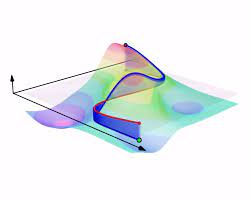
\includegraphics[scale=0.5]{figuras/imagen}
\vfill
BRYAN RICARDO BARBOSA OLVERA \\
\today \\

\end{center}
\end{titlepage}

\section{Introduccion}
\subsection{ Paquete de terceros }
//Crear un manejador de modulos  \\
go mod init holamundo
//Descargar un paquete \\
go get rxc.io/quote

\section{Uso de variables y datos}
\subsection{Declaracion de Variables}
\begin{verbatim}
    package main

import "fmt"

func main() {
	//Declaracion de variables
	//Forma 1
	var firstName, lastName string
	var age int
	firstName = "Bryan"
	lastName = "Ricardo"
	age = 27
	fmt.Println(firstName, lastName, age)

	/*
		//FORMA 2
		var (
			firstName , lastName string
			age int
		)
		firstName = "Bryan"
		lastName = "Ricardo"
		age = 27
		//FORMA 3
		var firstName, lastName, age = "Bryan", "Ricardo", 19
		//FORMA 4
		firstName, lastName, age:= "Bryan", "Ricardo", 19
	*/
}

\end{verbatim}

\newpage

\subsection{Declaracion de constantes}
\begin{verbatim}
package main

import "fmt"

//Declarar constantes

const Pi = 3.14

// Declarar varias constantes
const (
	x = 100
	y = 0b1010 //binario
	z = 0o12   //Octal
	w = 0xFF   //Hexadecimal
)

const (
	Domingo = iota + 1
	Lunes
	Martes
	Miercoles
	Jueves
	Viernes
	Sabado
)

func main() {
	fmt.Println(Pi)
	fmt.Println(x)
	fmt.Println(y)
	fmt.Println(z)
	fmt.Println(w)
	fmt.Println(Viernes)
}
\end{verbatim}
\subsection{Tipos de datos Basicos}

\begin{verbatim}
package main

import "fmt"

//TIPOS DE DATOS

func main() {

	var integer int8 = 127     //ENteros de 8 bits
	var integer2 uint8 = 127   //Enteros no  negativos de 8bits
	var float float32 = 9.8    // Tambien existe flaot64
	var valuesBool bool = true //Valor booleano
	fullName := "Bryan Ricardo \t (alias \" rinux\" ) \n"
	fmt.Println(fullName)
	var valorByte byte = 'a'

	s := "Hola"
	fmt.Println(s[0]) //Imprime el byte
}
\end{verbatim}

\newpage
\subsection{Conversion de datos}
\begin{verbatim}
package main

import (
	"fmt"
	"strconv"
)

//TIPOS DE DATOS

func main() {

	//Conversion de enteros y flotantes
	var integer16 int16 = 50
	var integer32 int32 = 100
	fmt.Println(int32(integer16) + integer32) //Es la misma logica de conversion para int y float

	//Convertir una cadena a un entero
	s := "100"
	i, _ := strconv.Atoi(s) //La barra es para no guardar el error
	fmt.Println(i + 10)

	//Conversio de enteros a cadenas
	n := 42
	s = strconv.Itoa(n) //Solo recibe te tipo int
	//Si es de tipo int8 es preferible convertilo a int
}
\end{verbatim}
\subsection{Funcion fmt}

\begin{verbatim}
package main

import (
	"fmt"
)

//TIPOS DE DATOS

func main() {

	var name string
	var age int
	fmt.Print("Ingrese su nombre: ")
	fmt.Scanln(&name) //Lee datos
	fmt.Print("Ingrese su edad: ")
	fmt.Scanln(&age)

	//Imprimir varios valores
	fmt.Printf("Hola, me llamo %s y tengo %d años.\n", name, age) //Si no se conoce el dato que se va ingresar se puede utilizar %v

	fmt.Printf("Los tipos de datos son: %T %T \n", name, age) //Si no se conoce el dato que se va ingresar se puede utilizar %v

}
\end{verbatim}
\newpage

\subsection{Paquete Math}

\begin{verbatim}
package main

import (
	"fmt"
	"math"
)

func main() {
	fmt.Println(math.Pi)
	fmt.Println(math.E)
	fmt.Println(math.Pow(2, 5)) //Potencia
	//Exiten aun mas funciones de math
}
\end{verbatim}

\section{Control de flujos}
\subsection{Declaracion If Else}
\begin{verbatim}
package main

import (
	"fmt"
	"time"
)

func main() {
	/*
	t := time.Now()
	hora := t.Hour()
	
	//METODO 1
	fmt.Println(t)
	fmt.Println(t.Hour())

	if hora < 12 {
		fmt.Println("Mañana")
	} else if hora < 17 {
		fmt.Println("Tarde")
	} else {
		fmt.Println("Noche")
	}
	*/
	
	//METODO 2
	if t:= hora < 12 {
		fmt.Println("Mañana")
	} else if hora < 17 {
		fmt.Println("Tarde")
	} else {
		fmt.Println("Noche")
	}
	
}
\end{verbatim}
\newpage
\subsection{Switch}

\begin{verbatim}
package main

import (
	"fmt"
	"runtime"
)

func main() {

	os := runtime.GOOS //Nos da el SO en el que se esta ejecutando

	switch os {
	case "windows":
		fmt.Println("Go run -> Windows")
	case "linux":
		fmt.Println("Go run -> Linux")
	case "darwin":
		fmt.Println("Go run -> Ios")
	default:
		fmt.Println("Go run -> Otro OS")
	}

}
\end{verbatim}

\subsection{For}
\begin{verbatim}
package main

import "fmt"

func main() {

	for i := 1; i <= 10; i++ {
		if i == 5 {
			//break se para aqui
			continue //Continua
		}
		fmt.Println(i)
	}

}
\end{verbatim}
\newpage
\subsection{Funciones}

\begin{verbatim}
package main

import "fmt"

func main() {

	saludo := hello("Bryan")
	fmt.Println(saludo)
	sum, mul := calc(4, 5)
	fmt.Println("La suma es: ", sum)
	fmt.Println("La multiplicacion es: ", mul)
}

func hello(name string) string /*Lo que va a retornar*/ {

	return "Hola, " + name
}

func calc(a, b int) (int, int) /*Devuelve dos valores enteros*/ {
	sum := a + b
	mul := a * b
	return sum, mul
}

/*
Forma 2
func calc(a, b int) (sum, mul int){}
	sum = a + b
	mul = a * b
	return sum, mul
}
*/
\end{verbatim}

\newpage
\section{Estructura de datos}
\subsection{Mátrices}

\begin{verbatim}
package main

import "fmt"

func main() {
	var a [5]int
	a[0] = 10
	a[1] = 10
	var b = [5]int{10, 20, 30, 40, 50}
	//var b = [...]int{10, 20, 30, 40, 50} Se usa cuando no sabemos la cantidad de datos que se van a guardar

	fmt.Println(a, b)
	for i := 0; i < len(b); i++ {
		fmt.Println(b[i])
	}

	//Forma 2 para iterar
	for index, value := range b {
		fmt.Printf("Indice: %d, Valor: %d \n ", index, value)
	}

	var matriz = [3][3]int{{1, 2, 3}, {4, 5, 6}, {7, 8, 9}}

	fmt.Println(matriz)

}
\end{verbatim}


\subsection{Rebandas}
\begin{verbatim}
package main

import "fmt"

func main() {
	diasSemana := []string{"Domingo", "Lunes", "Martes", "Miercoles", "Jueves", "Viernes", "Sabado"}
	diaRebanada := diasSemana[0:5]

	//Agregar elementos
	diaRebanada = append(diaRebanada, "Viernes", "Sabado")
	fmt.Println(diaRebanada)

	//Quitar elementos
	diaRebanada = append(diaRebanada[0:2], diaRebanada[3:]...)

	fmt.Println(diaRebanada)
	fmt.Println(len(diaRebanada))
	fmt.Println(cap(diaRebanada)) //Capacidad que puede guardar

	//Crear rebanadas con la palabra make
	nombres := make([]string, 5, 10)
	nombres[0] = "Bryan"
	fmt.Println(nombres)
	//Copiando los elementos con la palabra copy
	rebanada1 := []int{1, 2, 3, 4, 5}
	rebanada2 := make([]int, 5)
	copy(rebanada2, rebanada1) //Retorna la cantidad de elementos que se han copeado

	fmt.Println(rebanada1)
	fmt.Println(rebanada2)
}

\end{verbatim}

\subsection{Mapas}
\begin{verbatim}
package main

import "fmt"

func main() {
	colors := map[string]string{
		"rojo":  "#FF0000",
		"verde": "#00FF00",
		"azul":  "#0000FF",
	}

	fmt.Println(colors)
	fmt.Println(colors["rojo"])
	//Agregar un nuevo elemento
	fmt.Println(colors["rojo"])
	colors["negro"] = "#000000"
	fmt.Println(colors)
	//Nota, lo ordena alfabeticamente en automatico

	//Verificar si existe
	valor, ok := colors["blanco"] //Verifica si existe
	//ok: retorna un valor de tipo bool
	if ok {
		fmt.Println("Si existe la clave: ", valor)
	} else {
		fmt.Println("No existe esta clave")
	}
	//Eliminar un elementto
	delete(colors, "azul")
	fmt.Println(colors)

	//Iterar los valores
	for clave, valor := range colors {
		fmt.Printf("Clave: %s, valor: %s \n", clave, valor)
	}

}
\end{verbatim}
\newpage
\subsection{Estructuras}
\begin{verbatim}
package main

import "fmt"

// Estructura
type Persona struct {
	nombre string
	edad   int
	correo string
}

func main() {

	var p Persona
	p.nombre = "Bryan"
	p.edad = 19
	p.correo = "bryanrifardo@gmail.com"

	/*
		FORMA 2
		p:= Persona{"Bryan", 19, "bryanrifardo@gmail.com"}
	*/

	fmt.Println(p)

}
\end{verbatim}

\subsection{Punteros y metodos}
\begin{verbatim}
package main

import "fmt"

type Persona struct {
	nombre string
	edad   int
	correo string
}

// Metodo
func (p *Persona) diHola() {
	fmt.Println("Hola, mi nombre es", p.nombre)
}

func main() {
	var x int = 10
	fmt.Println(x)

	editar(&x) //ENviar la referencia de la memoria
	fmt.Println(x)

	//Crear una instancia del metodo
	p := Persona{"Bryan", 19, "bryanrifardo@gmail.com"}
	p.diHola()
}

func editar(x *int) {
	*x = 20
}
\end{verbatim}

\section{Control de errores}
\subsection{Manejo de errores}
\begin{verbatim}
package main

import (
	"errors"
	"fmt"
)

// Creando una funcion que puede enviar un error
func divide(dividendo, divisor int) (int, error) {
	if divisor == 0 {
		return 0, errors.New("No se puede dividir por 0")
		/*SEGUNDA FORMA
		return 0, fmt.Errorf("No se puede dividir por 0")
		*/
	}
	return dividendo / divisor, nil
}

func main() {
	/*
		EJemplo de un manejo de un error
		str := "123f"
		num, err := strconv.Atoi(str)
		//Manejar un error
		if err != nil {
			fmt.Println("Error", err)
			return
		}

		fmt.Println("Número:", num)
	*/
	//Lammando la funcion divide
	result, err := divide(10, 0)
	if err != nil {
		fmt.Println("Error:", err)
		return
	}
	fmt.Println("Resultado: ", result)
}

\end{verbatim}
\newpage
\subsection{Defer}
\begin{verbatim}
package main

import (
	"fmt"
	"os"
)

func main() {
	/*defer fmt.Println(3) //Posponer una  ejecucion
	defer fmt.Println(2)
	defer fmt.Println(1)
	*/
	file, err := os.Create("hola.txt") //Crea un archivo
	if err != nil {
		fmt.Println(err)
		return
	}

	defer file.Close()
	/*
		Lo enterior se puede utilizar para cerrar el flujo, tambien
		se utiliza para cerrar una base de datos
	*/

	_, err = file.Write([]byte("Hola, Bryan Ricardo"))
	if err != nil {
		fmt.Println(err)
		return
	}

}
\end{verbatim}
\subsection{Panic y Recover}

\begin{verbatim}

package main

import "fmt"

func divide(dividiendo, divisor int) {

	//Capturar el error sin interferir en el programa
	defer func() { //Funcion anonima
		if r := recover(); r != nil {
			fmt.Println(r)
		}
	}()

	validateZero(divisor)
	fmt.Println(dividiendo / divisor)
}
func validateZero(divisor int) {
	if divisor == 0 {
		panic("No puedes dividir por cero") //Cuando se ejecuta
		//Entra en un modo de panico, pero se ejecuta lo anterior
		//Proboca un panico cuando ocurre un error
	}
}

func main() {
	divide(100, 10)
	divide(200, 25)
	divide(34, 0)
	divide(100, 4)
}
\end{verbatim}
\subsection{Registro de errores}
\begin{verbatim}
package main

import (
	"log"
	"os"
)

func main() {
	//log.Fatal("¡Oye, soy un registro de errores!")
	//Imprime el registro pero detiene el programa
	//log.Panic("Panico")
	//Imprime el panico pero detiene el programa

	//Guardar errores

	file, err := os.OpenFile("info.log", os.O_CREATE|os.O_APPEND|os.O_WRONLY, 0644)
	if err != nil {
		log.Fatal(err)
	}

	defer file.Close()
	log.SetOutput(file)
	log.Print("¡Oye,soy un Log")

}
\end{verbatim}
\newpage
\section{Crear un modulo-Proyecto}
1.mkdir greetings \\
2.cd greetings/  \\
3.go mod init github.com/Bryan-Ricardo/greetings //Creando el manejador de modulos \\
4.nvim greetings.go //Creando un archivo .go \\
5.Escribir lo siguiente: \\
\begin{verbatim}
package greetings

import "fmt"

//Hello

func Hello(name string) string {
	message := fmt.Sprintf("¡Hola, %v! ¡Bienvenido!", name)
	return message
}

\end{verbatim}

6.Salir del documento \\
7.Ejecutar cd .. \\para salir de la carpeta \\
8.mkdir hello \\ 
9.cd hello \\
10.go mod init hello \\
11.nvim main.go \\
12. Escribir lo siguiente 
\begin{verbatim}
package main
import (
	"fmt"

	"github.com/Bryan-Ricardo/greetings"
)

func main() {
	message := greetings.Hello("Bryan")
	fmt.Println("vim-go")
}

\end{verbatim}

13.Salir del documento \\ 
14.go mod edit -replace github.com/Bryan-Ricardo/greetings=../greetings\\
15.go mod tidy // Guardar los cambios \\
16.go run //Ejecutar el programa

\newpage

\subsection{Agregar un manejador de errores}
1.En el archivo greetings: 

\begin{verbatim}
package greetings

import (
	"errors"
	"fmt"
)

//Hello
func Hello(name string) (string, error) {

	if name == "" {
		return "", errors.New("Nombre vacío")
	}

	message := fmt.Sprintf("¡Hola, %v! ¡Bienvenido!", name)
	return message, nil
}
\end{verbatim}

2.En el archivo hello: 

\begin{verbatim}
package main

import (
	"fmt"
	"log"

	"github.com/Bryan-Ricardo/greetings"
)

func main() {
	log.SetPrefix("greetings: ")
	log.SetFlags(0)

	message, err := greetings.Hello("")
	if err != nil {
		log.Fatal(err)
	}
	fmt.Println(message)
}
\end{verbatim}

\newpage
\subsection{Devolver un saludo aleatorio}
1.Escribir lo siguiente en greetings
\begin{verbatim}
package greetings

import (
	"errors"
	"fmt"
	"math/rand"
)

//Hello

func Hello(name string) (string, error) {

	if name == "" {
		return "", errors.New("Nombre vacío")
	}

	message := fmt.Sprintf(randomFormat(), name)
	return message, nil
}

func randomFormat() string {

	formats := []string{
		"¡Hola, %v! ¡Bienvenido",
		"¡Qué bueno verte, %v!",
		"¡Saludo, %v! ¡Encantado de conocerte!",
	}

	return formats[rand.Intn(len(formats))]

}
\end{verbatim}
\newpage
\section{POO e Interfaces }
\subsection{Estructuras y metodos}
1.mkdir library \\
2.go mod init library \\
3.nvim main \\
4.mkdir book \\
5.cd book \\
6.nvim book \\
7.Escribir en book lo siguiente: 
\begin{verbatim}
package book

import "fmt"

type Book struct {
	Title  string
	Author string
	Pages  int
}

// Creando el "Constructor"
func NewBook(title string, author string, pages int) *Book {

	return &Book{
		Title:  title,
		Author: author,
		Pages:  pages,
	}

}

func (b *Book) PrintInfo() {

	fmt.Printf(" Title: %s\n Author: %s \n Pages: %d \n", b.Title, b.Author, b.Pages)

}
\end{verbatim}
8.Escribir en main lo siguiente: 
\begin{verbatim}
    package main

import (
	"library/book"
)

func main() {
	/*
		Primera forma sin el contructor
		var myBook = book.Book{
			Title:  "Mody Dick",
			Author: "Herman Melville",
			Pages:  300,
		}

		myBook.PrintInfo()
	*/
	//SEGUNDA FORMA CON EL CONSTRUCTOR
	myBook := book.NewBook("Mody Dick", "Herman Melville", 300)
	myBook.PrintInfo()
}
\end{verbatim}

\end{document}
